\section{Análisis de Resultados con ACAMD}\label{analisis_resultados_acamd}
La metodología ACAMD, introducida en la sección anterior, será ahora aplicada para desentrañar las complejidades detrás del éxito académico de los estudiantes.\footnote{El código fuente y los notebooks de Jupyter utilizados en este análisis están disponibles en \url{https://github.com/tonporaqui/tesis}} Esta metodología única, que combina las fortalezas de SHAP para la interpretación de modelos y DoWhy para el análisis causal, nos permitirá no solo identificar las variables más influyentes, sino también entender las relaciones causales que existen entre ellas. A continuación, exploraremos cómo ACAMD ilumina nuestro análisis de los datos del año 2021.

El análisis se centra en \texttt{sol1}, identificada como nuestra variable clave. Utilizando SHAP, evaluamos la influencia de \texttt{sol1} en el rendimiento académico, seguido de la construcción de un modelo causal con DoWhy. Este enfoque responde a nuestra pregunta central de investigación: ¿Cómo se relaciona la resolución de una guía de programación con el éxito académico en el curso introductorio de programación en la Universidad Andrés Bello?

A través de ACAMD, no solo validamos la relevancia de \texttt{sol1} sino que también descubrimos las relaciones causales potenciales entre la participación activa de los estudiantes en las guías de programación y sus logros académicos. Estos hallazgos son fundamentales para el desarrollo de estrategias pedagógicas efectivas y la optimización de las guías como herramientas educativas.



\subsection{Análisis de datos}

Tras la recopilación de datos, se efectuará un análisis descriptivo para inspeccionar la distribución de los resultados tanto en la guía de programación como en la primera evaluación. Adicionalmente, se realizará un análisis de correlación entre las variables previamente mencionadas con el fin de discernir relaciones y patrones significativos.

\subsubsection{Descripción de la base de datos}

A continuación, se detalla la estructura de la base de datos:

\begin{table}[H]
    \centering
    \caption{Descripción de variables}
    \begin{tabular}{lp{0.6\linewidth}}
        \toprule
        \textbf{Variable} & \textbf{Descripción} \\
        \midrule
        sol1 & Nota en la primera evaluación (rango 0-7) \\
        exitosos & Cantidad de respuestas correctas en la guía \\
        fallidos & Número de intentos en la guía \\
        hito1 hito2 & Expectativas de aprendizaje del curso (conjunto de preguntas) \\
        programa & Programa académico del estudiante \\
        Columnas e0 hasta la e52 & Resultados de la guía (1: correcto, 0: incorrecto) \\
        \bottomrule
    \end{tabular}
    \label{tab:variables}
\end{table}

Las columnas descritas son esenciales para nuestro análisis, ya que nos facilitan la exploración de la relación entre la resolución de la guía de programación, el rendimiento académico en la primera evaluación y el programa académico del estudiante (véase Tabla \ref{tab:variables}).

\subsubsection{Variable Objetivo}

El propósito principal de esta investigación es determinar la influencia de la resolución de la guía en el desempeño de la evaluación del curso. Por ello, se propone la variable \textit{sol1} como variable objetivo. Dado su carácter cuantitativo, se recomienda añadir una columna denominada \textit{aprobado}, de naturaleza binaria. En esta columna, se asignará el valor 1 a las notas que oscilen entre 4.0 y 7.0, y el valor 0 a las notas inferiores, denotando la condición de reprobado. Esta transformación se ilustra en el siguiente fragmento de código:

\begin{lstlisting}[language=Python, caption=Tratamiento de la Variable Objetivo ,label=lst:trat_varObjetivo]
    # Creación de la columna 'aprobado' y población de la misma.
    df["aprobado"] = df.apply(lambda x: functions.set_in_aprobado_nota(x["sol1"]), axis=1)
\end{lstlisting}

\subsubsection{Descripción del DataFrame}

La Tabla \ref{tab:descripcion_dataframe} ofrece un resumen del DataFrame, detallando las columnas, la cantidad de valores no nulos y los tipos de datos asociados. Esta descripción brinda una perspectiva general de la estructura y características del DataFrame.

\begin{table}[H]
    \centering
    \caption{Descripción del DataFrame}
    \begin{tabular}{lll}
        \hline
        \textbf{Columna} & \textbf{Non-Null Count} & \textbf{Dtype} \\
        \hline
        hito1            & 839 non-null            & float64        \\
        hito2            & 839 non-null            & float64        \\
        exitosos         & 839 non-null            & int64          \\
        fallidos         & 839 non-null            & int64          \\
        sol1             & 839 non-null            & float64        \\
        aprobado         & 839 non-null            & int64          \\
        e0 - e52         & 839 non-null            & int64          \\
        \hline
    \end{tabular}%
    \label{tab:descripcion_dataframe}%
\end{table}%

Como se observa en la Tabla \ref{tab:descripcion_dataframe}, cada columna cuenta con 839 valores no nulos y se especifica el tipo de dato correspondiente. Estos detalles son cruciales para entender la composición y propiedades del DataFrame en estudio.

\subsubsection{Estadísticas de la variable objetivo}

Dentro del análisis de datos, es esencial conocer las características estadísticas de las variables numéricas. En este contexto, se ha examinado la variable \textit{sol1}, recopilando estadísticas como el recuento, la media, la desviación estándar, los cuartiles y el sesgo. Estos valores ofrecen una visión sobre la distribución y tendencia central de la variable.

\begin{table}[H]
    \centering
    \caption{Estadísticas de la variable objetivo}
    \begin{tabular}{ll}
        \hline
        \textbf{Medida}    & \textbf{Valor}       \\
        \hline
        Count              & 839.000000           \\
        Mean               & 3.642789             \\
        Standard Deviation & 1.832625             \\
        Minimum            & 1.000000             \\
        25\% Percentile    & 2.200000             \\
        50\% Percentile    & 3.700000             \\
        75\% Percentile    & 5.100000             \\
        Maximum            & 7.000000             \\
        Skewness           & 0.033079652062595215 \\
        \hline
    \end{tabular}%
    \label{tab:estadistica_variable_sol1}%
\end{table}%

La Tabla \ref{tab:estadistica_variable_sol1} revela que la variable \textit{sol1} tiene una media cercana a 3.6 y una desviación estándar alrededor de 1.83. La distribución de los datos muestra un ligero sesgo positivo con un valor de aproximadamente 0.03. Estos resultados nos permiten entender la variabilidad y forma de la distribución de la variable \textit{sol1}.

\subsubsection{Coeficiente de asimetría de la variable objetivo}

El coeficiente de asimetría es una métrica que brinda información sobre la asimetría de una distribución de datos. Para los datos analizados, se ha obtenido un coeficiente de asimetría de aproximadamente 3.31\%. Este valor señala una ligera asimetría positiva en la distribución.

\begin{table}[H]
    \centering
    \caption{Coeficiente de asimetría}
    \begin{tabular}{ll}
        \hline
        \textbf{Coeficiente de asimetría}      & \textbf{Valor}       \\
        \hline
        Coeficiente de asimetría               & 0.033079652062595215 \\
        Coeficiente de asimetría en porcentaje & 3.31\%               \\
        \hline
    \end{tabular}%
    \label{tab:skewness}%
\end{table}%

La Tabla \ref{tab:skewness} muestra un coeficiente de asimetría de 0.033079652062595215, lo que indica una ligera asimetría hacia la derecha. Esto sugiere que hay una cola derecha más extensa en comparación con la cola izquierda de la distribución. En términos porcentuales, esta asimetría representa aproximadamente el 3.31\% del rango total de la distribución.

\subsubsection{Coeficiente de Variación de la variable objetivo}

El coeficiente de variación es una métrica que refleja la dispersión relativa de una variable respecto a su media. Facilita la evaluación de la variabilidad de los datos en relación con su valor medio. Se calcula dividiendo la desviación estándar entre la media y se expresa en porcentaje.

\begin{table}[H]
    \centering
    \caption{Coeficiente de Variación}
    \begin{tabular}{ll}
        \hline
        \textbf{Medida}                        & \textbf{Valor}     \\
        \hline
        Coeficiente de Variación               & 0.5027829289053924 \\
        \hline
        Coeficiente de Variación en Porcentaje & 50.28\%            \\
        \hline
    \end{tabular}%
    \label{tab:coef_variacion}%
\end{table}%

La Tabla \ref{tab:coef_variacion} muestra el coeficiente de variación calculado para los datos analizados. Este coeficiente es de aproximadamente 0.5027, lo que indica una alta dispersión relativa respecto a la media. Esto se confirma con el coeficiente de variación en porcentaje, que es del 50.28\%. Estos resultados subrayan la variabilidad de los datos en el conjunto analizado.

\subsubsection{Amplitud de la variable objetivo}

La amplitud es una métrica que refleja la variabilidad o dispersión de los datos. Permite evaluar la diferencia entre el valor máximo y mínimo de una variable, proporcionando información sobre la extensión de los datos en el conjunto.

\begin{table}[H]
    \centering
    \caption{Amplitud}
    \begin{tabular}{ll}
        \hline
        \textbf{Medida} & \textbf{Valor}     \\
        \hline
        Amplitud        & 0.5600809456082252 \\
        \hline
    \end{tabular}%
    \label{tab:amplitud}%
\end{table}%

La Tabla \ref{tab:amplitud} muestra la amplitud calculada para los datos analizados. La amplitud es de aproximadamente 0.56\%, lo que indica la diferencia entre el valor máximo y mínimo de la variable. Esta métrica nos proporciona una idea de la extensión de los datos en el conjunto analizado.

\subsubsection{Tabla de Frecuencias de la variable objetivo}

Utilizando los datos de la Tabla \ref{tab:skewness} y la Tabla \ref{tab:amplitud}, se ha elaborado una tabla de frecuencias que refleja la distribución de los datos en intervalos. Los intervalos se definen en función de la amplitud y el valor máximo de los datos.

\begin{table}[H]
    \centering
    \caption{Tabla de Frecuencias}
    \begin{tabular}{lllll}
        \hline
        \textbf{Intervalo} & \textbf{f\_i} & \textbf{F\_i} & \textbf{h\_i} & \textbf{H\_i} \\
        \hline
        (0.0, 0.56]        & 0             & 0             & 0.000000      & 0.000000      \\
        (0.56, 1.12]       & 152           & 152           & 0.181168      & 0.181168      \\
        (1.12, 1.68]       & 21            & 173           & 0.025030      & 0.206198      \\
        (1.68, 2.24]       & 66            & 239           & 0.078665      & 0.284863      \\
        (2.24, 2.8]        & 79            & 318           & 0.094160      & 0.379023      \\
        (2.8, 3.36]        & 34            & 352           & 0.040524      & 0.419547      \\
        (3.36, 3.92]       & 103           & 455           & 0.122765      & 0.542312      \\
        (3.92, 4.48]       & 76            & 531           & 0.090584      & 0.632896      \\
        (4.48, 5.04]       & 87            & 618           & 0.103695      & 0.736591      \\
        (5.04, 5.6]        & 81            & 699           & 0.096544      & 0.833135      \\
        (5.6, 6.16]        & 53            & 752           & 0.063170      & 0.896305      \\
        (6.16, 6.72]       & 57            & 809           & 0.067938      & 0.964243      \\
        \hline
    \end{tabular}%
    \label{tab:tabla_frecuencias}%
\end{table}%

La Tabla \ref{tab:tabla_frecuencias} presenta la tabla de frecuencias que muestra la cantidad de datos en cada intervalo, el total acumulado de datos hasta ese intervalo, la frecuencia relativa del intervalo y la frecuencia relativa acumulada. Esta tabla nos permite visualizar la distribución de los datos y su acumulación en cada intervalo.

El intervalo más relevante es (3.36, 3.92], ya que contiene la mayor frecuencia (103) y la mayor acumulación (455). Esto indica que la mayoría de los datos se encuentran en este rango.

A continuación, se presenta una tabla con información adicional:

\begin{table}[H]
    \centering
    \caption{Información Adicional}
    \begin{tabular}{lllll}
        \hline
        \textbf{Mediana} & \textbf{Intervalo de la mediana} & \textbf{Máximo} & \textbf{Intervalo del máximo} \\
        \hline
        3.7              & $f_i$ 103.000000                 & 7.0             & $f_i$ 57.000000               \\
                         & $F_i$ 455.000000                 &                 & $F_i$ 809.000000              \\
                         & $h_i$ 0.122765                   &                 & $h_i$ 0.067938                \\
                         & $H_i$ 0.542312                   &                 & $H_i$ 0.964243                \\
        \hline
    \end{tabular}%
    \label{tab:informacion_adicional}%
\end{table}%

La Tabla \ref{tab:informacion_adicional} muestra la mediana de los datos y el intervalo en el que se encuentra. También se indica el valor máximo y el intervalo correspondiente.

\subsubsection{Histograma con curva de densidad de la variable objetivo}

El histograma con curva de densidad es una herramienta visual que permite comprender la distribución de los valores de la variable \textit{sol1}.

\begin{figure}[H]
    \centering
    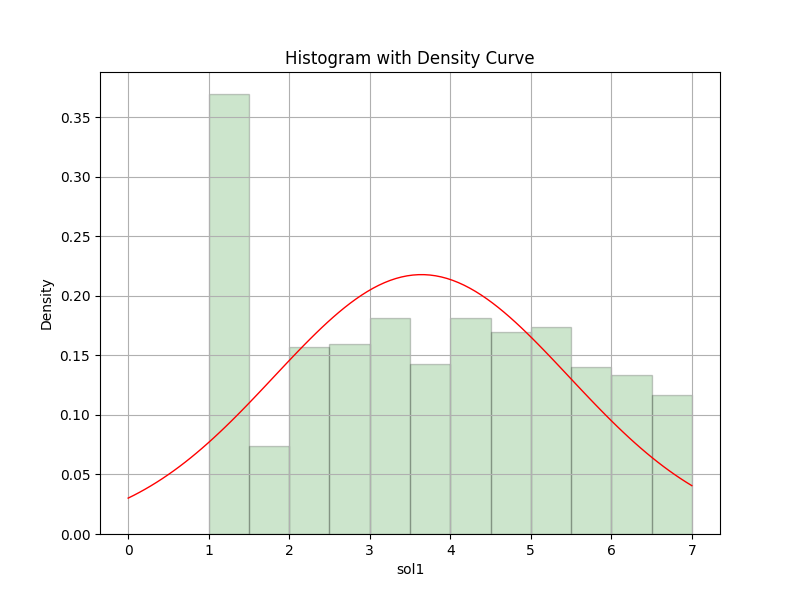
\includegraphics[width=4.06111in,height=2.68611in]{img/histogramaConCurvaDeDensidad.png}
    \caption{Histograma con Curva de Densidad}
    \label{fig:hist_density}%
\end{figure}%

La Figura \ref{fig:hist_density} muestra el histograma con curva de densidad correspondiente a los datos analizados. En el eje Y, se presentan los valores de densidad, mientras que en el eje X, se muestran las notas obtenidas en \textit{sol1}. La mayor concentración de datos se encuentra alrededor del valor 0.35 en el eje Y, lo que indica que la mayoría de las observaciones tienen una nota baja en \textit{sol1}. La curva de densidad, representada en rojo, alcanza su punto más alto entre las notas 3 y 4 en el eje X. Esta curva suavizada muestra la forma general de la distribución de los valores de \textit{sol1}. A medida que las notas aumentan, la densidad disminuye gradualmente.

\subsubsection{Identificación de valores atípicos de la variable objetivo}

La detección de valores atípicos es esencial en el análisis de datos para identificar observaciones que se desvían significativamente de la tendencia general. Estos valores pueden tener un impacto significativo y requerir un análisis más detallado.

A continuación, se muestra una tabla con los valores atípicos identificados mediante el método del Z-score:

\begin{table}[H]
    \centering
    \caption{Valores Atípicos}
    \begin{tabular}{ccccccc}
        \hline
        \textbf{hito1} & \textbf{hito2} & \textbf{exitosos} & \textbf{fallidos} & \textbf{programa} & \textbf{sol1} & \textbf{aprobado} \\
        21.0           & 6.0            & 17                & 14                & UNAB11500         & 1.0           & 0                 \\
        2.0            & 2.0            & 4                 & 27                & UNAB12210         & 1.0           & 0                 \\
        4.0            & 4.0            & 6                 & 41                & UNAB12510         & 1.5           & 0                 \\
        0.0            & 0.0            & 0                 & 47                & UNAB12100         & 1.6           & 0                 \\
        10.0           & 6.0            & 9                 & 38                & UNAB11500         & 1.6           & 0                 \\
        12.0           & 0.0            & 9                 & 38                & UNAB12210         & 2.4           & 0                 \\
        42.0           & 12.0           & 26                & 37                & UNAB21500         & 2.5           & 0                 \\
        32.0           & 32.0           & 26                & 5                 & UNAB11500         & 3.4           & 0                 \\
        9.0            & 0.0            & 7                 & 40                & UNAB11500         & 4.3           & 1                 \\
        38.0           & 6.0            & 28                & 35                & UNAB12210         & 4.4           & 1                 \\
        32.0           & 32.0           & 26                & 5                 & UNAB12210         & 4.6           & 1                 \\
        18.0           & 2.0            & 11                & 20                & UNAB12210         & 4.6           & 1                 \\
        32.0           & 14.0           & 21                & 10                & UNAB12210         & 5.9           & 1                 \\
        13.0           & 25.0           & 16                & 15                & UNAB22115         & 7.0           & 1                 \\
        7.0            & 0.0            & 5                 & 42                & UNAB12100         & 7.0           & 1                 \\
        \hline
    \end{tabular}%
    \label{tab:valores_atipicos}%
\end{table}%

Observando los valores atípicos en la tabla \ref{tab:valores_atipicos}, podemos notar que algunas observaciones difieren significativamente en al menos una de las variables. \say{exitosos} representa las respuestas correctas de la guía, \say{fallidos} indica la cantidad de errores para lograr los \say{exitosos}, \say{programa} se refiere a la carrera a la cual pertenece. \say{sol1} se refiere a la nota obtenida en la solemne, \say{aprobado} se refiere si la nota de solemen es mayor mayor o igual a 4 el alumno es aprobado(columna agregada por medio de script). Estos valores atípicos pueden ser de interés para un análisis más detallado, ya que podrían indicar situaciones excepcionales o errores en la recolección de datos.

\subsection{Comparación de algoritmos}

En esta sección, comparamos varios algoritmos con respecto a nuestras métricas de interés: Accuracy, Precision, Recall y F1 Score (R2). Los algoritmos considerados se dividen en:

% -----------

\subsubsection{Comparacion y Analisis de Modelos de Clasificación}

\begin{itemize}
    \item DecisionTreeClassifier
    \item LogisticRegression
    \item RandomForestClassifier
    \item XGBClassifier
\end{itemize}

Para estos modelos, se utilizará la variable objetivo \say{aprobado}, la técnica \say{Stratified K-Fold Cross-Validation}, ajustaremos el mejor modelo en los datos de entrenamiento y realizaremos predicciones utilizando el mejor modelo.

La mejor configuración para los modelos de clasificación se muestra en el siguiente codigo: \ref{lst:config_clasificacion}:


\begin{lstlisting}[language=Python, caption=Definicion de los Modelos de Clasificación,label=lst:config_clasificacion]
    # Definir los modelos de Clasificacion
    models_clasificacion = [
        DecisionTreeClassifier(
            min_samples_split=10,
            min_samples_leaf=5,
        ),
        LogisticRegression(penalty="l2", C=1.0, solver="lbfgs", max_iter=150),
        RandomForestClassifier(
            max_depth=10,
            min_samples_split=10,
            min_samples_leaf=5,
            random_state=1502,
            n_estimators=500,
        ),
        XGBClassifier(learning_rate=0.1, max_depth=10, n_estimators=150, subsample=1.0),
    ]
\end{lstlisting}

% -----------

\subsubsection{Determinación de Características Clave y Variable Objetivo para Modelos de Clasificación}

En el siguiente fragmento de código, se lleva a cabo el proceso de selección de características relevantes para los modelos de clasificación. La variable objetivo, denominada aprobado, indica si un estudiante ha aprobado o no. Las características seleccionadas, representadas por X, incluyen diversos indicadores y hitos del estudiante, como hito1, hito2, y eventos específicos e0 a e52. Estas características se extraen del dataframe df y se utilizarán para entrenar y evaluar los modelos de clasificación.

\begin{lstlisting}[language=Python, caption=Selección de características y variable objetivo, label=lst:seleccion_caracteristicas]
y = df["aprobado"]
X = df[
['hito1', 'hito2', 'exitosos', 'fallidos','e0', 'e1', 'e2', 'e3', 'e4', 'e5', 'e6', 'e7', 'e8', 'e9', 'e10', 'e11', 'e12', 'e13', 'e14', 'e15', 'e16', 'e17', 'e18', 'e19', 'e20', 'e21', 'e22', 'e23', 'e24', 'e25', 'e26', 'e27', 'e28', 'e29', 'e30', 'e31', 'e32', 'e33', 'e34', 'e35', 'e36', 'e37', 'e38', 'e39', 'e40', 'e41', 'e42', 'e43', 'e44', 'e45', 'e46', 'e47', 'e48', 'e49', 'e50', 'e51', 'e52']
]
\end{lstlisting}

% -----------

\subsubsection{Validación Cruzada Estratificada y Ajuste de Modelos de Clasificación}

En el siguiente fragmento de código, se establece un proceso de validación cruzada estratificada para evaluar varios modelos de clasificación. Primero, definimos las métricas de interés: precisión, exhaustividad, exactitud y la puntuación F1. Luego, aplicamos la técnica de Stratified K-Fold Cross-Validation para garantizar que cada pliegue sea una buena representación del conjunto de datos completo. A continuación, entrenamos cada modelo y evaluamos su rendimiento utilizando las métricas definidas. Finalmente, identificamos y mostramos el modelo con el mejor rendimiento promedio.

\begin{lstlisting}[language=Python, caption=Aplicación de Stratified K-Fold y entrenamiento de modelos, label=lst:stratified_kfold]
    # Definir las métricas
    metrics = ["accuracy", "precision", "recall", "f1"]

    # Realizar Stratified K-Fold Cross-Validation en los datos de entrenamiento y obtener las métricas para cada modelo
    results_train = (
        {}
    )  # Diccionario para almacenar los resultados de entrenamiento de cada modelo

    for model in models_clasificacion:
        model_name = model.__class__.__name__

        cv = StratifiedKFold(n_splits=10, shuffle=True, random_state=1502)
        # Dividir los datos en conjuntos de entrenamiento y prueba
        X_train, X_test, y_train, y_test = train_test_split(
            X, y, test_size=0.2, random_state=1502
        )

        model.fit(X_train, y_train)  # Ajustar el modelo en los datos de entrenamiento
        model_results = (
            {}
        )  # Diccionario para almacenar los resultados de las métricas para el modelo actual

        # Calcular las métricas utilizando validación cruzada
        for metric in metrics:
            scores = cross_val_score(model, X_train, y_train, cv=cv, scoring=metric)
            model_results[metric] = scores

        results_train[
            model_name
        ] = model_results  # Almacenar los resultados del modelo en el diccionario

    best_model = None
    best_score = 0.0

    # Encontrar el mejor modelo basado en la media de las métricas
    for model_name, model_result in results_train.items():
        mean_scores = [np.mean(model_result[metric]) for metric in metrics]
        mean_score = np.mean(mean_scores)

        if mean_score > best_score:
            best_score = mean_score
            best_model = model_name

    # Imprimir el mejor modelo y su puntuación
    print("El mejor modelo en la validación fue:", best_model, best_score)
\end{lstlisting}

% -----------

\subsubsection{Resultados de la Validación Cruzada Estratificada}

Después de aplicar la validación cruzada estratificada y entrenar los modelos de clasificación, se evaluaron sus rendimientos utilizando varias métricas. El modelo que demostró tener el mejor rendimiento promedio fue el RandomForestClassifier, con una puntuación de 0.6433 (redondeado a cuatro decimales). Esta puntuación se calculó como el promedio de las métricas de precisión, exhaustividad, exactitud y la puntuación F1.

Con estos resultados, se destaca la eficacia del modelo de clasificación basado en bosques aleatorios para este conjunto de datos en particular, lo que sugiere que puede ser una opción adecuada para futuras predicciones o análisis relacionados.

\begin{lstlisting}[language=Python, caption=Resultado Mejor modelo en la Validacion de Clasificación, label=lst:rest_bestModelClasification]
    El mejor modelo en la validación fue: RandomForestClassifier 0.6432621955500205
    \end{lstlisting}



% -----------

\subsubsection{Predicciones con el Mejor Modelo en el Conjunto de Prueba}

En el siguiente fragmento de código, buscamos el objeto correspondiente al mejor modelo identificado previamente, en este caso, el RandomForestClassifier. Una vez encontrado, ajustamos este modelo utilizando el conjunto de entrenamiento y luego realizamos predicciones sobre el conjunto de prueba. Posteriormente, calculamos métricas clave, como el Mean Squared Error (MSE) y el R2 Score, para evaluar el rendimiento del modelo en el conjunto de prueba.

\begin{lstlisting}[language=Python, caption=Predicciones y evaluación del mejor modelo, label=lst:prediccion_mejor_modelo]
    best_model_search = None

    # Buscar el objeto del mejor modelo en la lista de modelos
    for model in models_clasificacion:
        if model.__class__.__name__ == best_model:
            best_model_search = model
            break
    
    best_model_search.fit(
        X_train, y_train
    )  # Ajustar el mejor modelo en los datos de entrenamiento
    y_pred = best_model_search.predict(
        X_test
    )  # Realizar predicciones utilizando el mejor modelo
    
    # Calcular y mostrar los resultados obtenidos del mejor modelo
    mse = mean_squared_error(y_test, y_pred)  # Calcular el Mean Squared Error
    r2 = r2_score(y_test, y_pred)  # Calcular el R2 Score
    
    print("Resultados del mejor modelo:", best_model, "en el conjunto de prueba:")
    print("Mean Squared Error:", mse)
    print("R2 Score:", r2)
    \end{lstlisting}

Después de realizar las predicciones con el RandomForestClassifier en el conjunto de prueba, obtuvimos los siguientes resultados:

Mean Squared Error (MSE): 0.3631 (redondeado a cuatro decimales)
R2 Score: 0.4532 (redondeado a cuatro decimales)

Estos resultados proporcionan una medida cuantitativa del rendimiento del modelo en el conjunto de prueba. Es importante notar que un R2 Score negativo indica que el modelo no es adecuado para predecir la variable objetivo en este conjunto de datos, y puede ser menos preciso que un modelo simple que siempre predice el valor medio.

% ------------

\subsubsection{Comparación Gráfica de Métricas de Rendimiento en Modelos de Clasificación (Conjunto de Entrenamiento)}

A continuación, se presentan los resultados obtenidos para el conjunto de entrenamiento. La Figura \ref{fig:metricas_clasificacion} ilustra las métricas de rendimiento de diversos modelos de clasificación evaluados.

\begin{figure}[H]
    \centering
    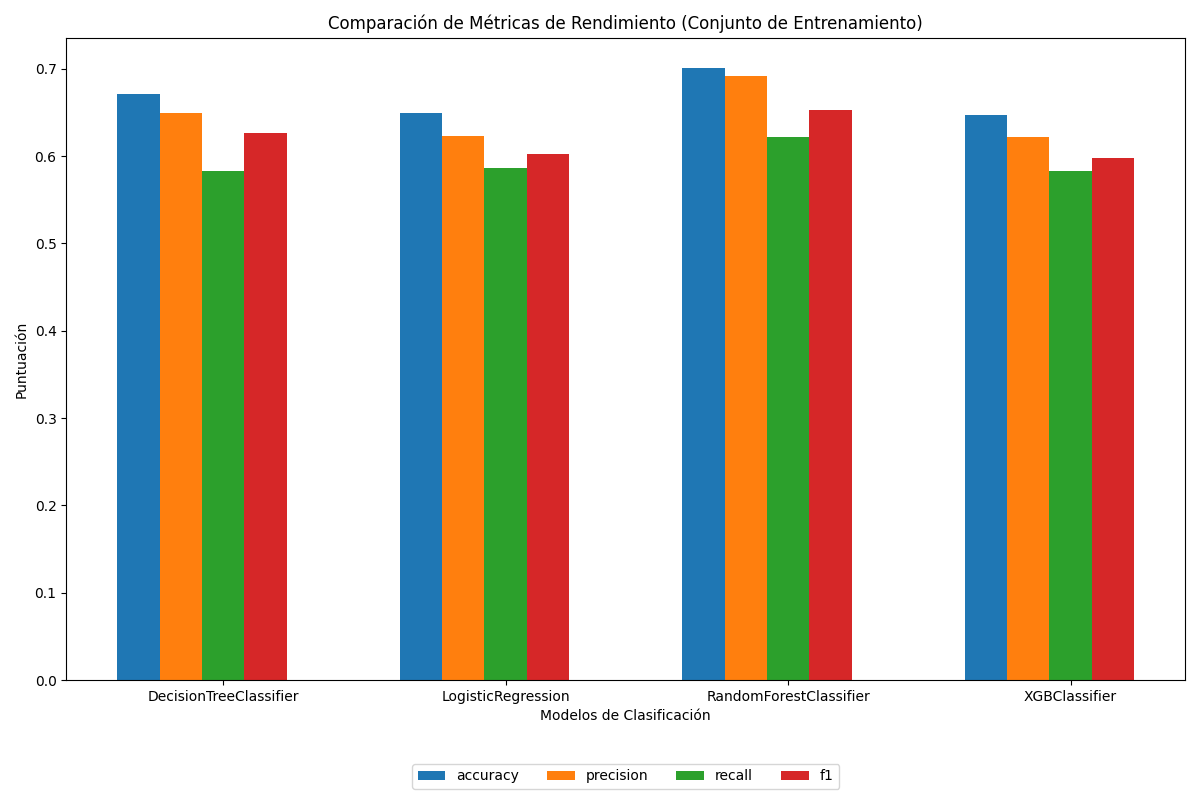
\includegraphics[width=1\textwidth]{img/compara_algoritmos/metricasEntreModelosClasificacion.png}
    \caption{Comparativa de métricas entre modelos de clasificación para el conjunto de entrenamiento.}
    \label{fig:metricas_clasificacion}
\end{figure}

La figura destaca que el modelo RandomForestClassifier sobresale en comparación con los otros modelos en todas las métricas evaluadas. En particular, este modelo logra un F1 Score de 62.53\%, un recall de 58.90\%, una precisión de 67.61\% y una exactitud de 66.54\%.

Para una visión más detallada y estructurada de estos resultados, se presenta la siguiente tabla:

\begin{table}[H]
    \centering
    \caption{Comparación de Métricas de Rendimiento para Modelos de Clasificación}
    \begin{tabular}{lcccc}
        \toprule
        \textbf{Modelo} & \textbf{Accuracy} & \textbf{Precision} & \textbf{Recall} & \textbf{F1} \\
        \midrule
        DecisionTreeClassifier & 0.6409 & 0.6300 & 0.5194 & 0.5708 \\
        LogisticRegression & 0.6617 & 0.6446 & 0.5792 & 0.6069 \\
        RandomForestClassifier & 0.6826 & 0.6761 & 0.5890 & 0.6253 \\
        XGBClassifier & 0.6186 & 0.5865 & 0.5262 & 0.5534 \\
        \bottomrule
    \end{tabular}
    \label{tab:performance_metrics}
\end{table}

Para el conjunto de prueba, los resultados se muestran en la Figura \ref{fig:metricas_clasificacion_bestModel}.

\begin{figure}[H]
    \centering
    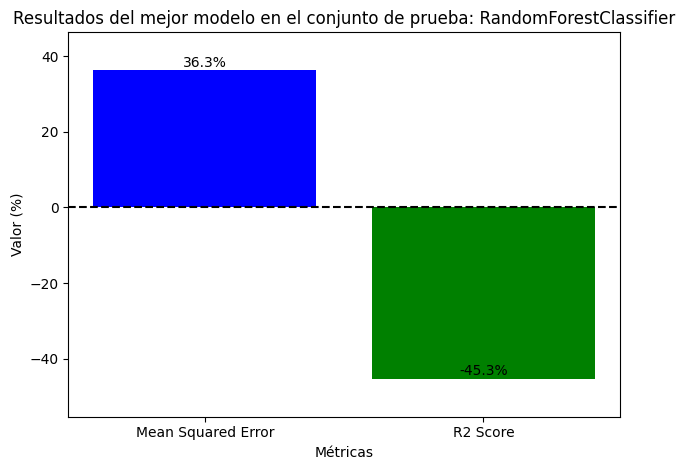
\includegraphics[width=0.8\textwidth]{img/compara_algoritmos/metricasBestModelRandomForesClassifier.png}
    \caption{Métricas del mejor modelo de clasificación en el conjunto de prueba.}
    \label{fig:metricas_clasificacion_bestModel}
\end{figure}

Las métricas cuantitativas para el conjunto de prueba son:

\begin{itemize}
    \item Mean Squared Error: 36.3\%
    \item R2 Score: -45.3\%
\end{itemize}

Con base en los resultados obtenidos, se concluye que el modelo RandomForestClassifier es el más adecuado para abordar este problema de clasificación. En la validación, este modelo demostró ser el mejor, con una puntuación del 62.53\%.

% -----------

\subsubsection{Comparacion y Analisis de Modelos de Regresión}

La regresión es una técnica estadística que permite modelar y analizar las relaciones entre una variable dependiente y una o más variables independientes.

\begin{itemize}
    \item LinearRegression
    \item DecisionTreeRegressor
    \item KNeighborsRegressor
\end{itemize}

Para estos modelos, se utilizará la variable objetivo \say{sol1}, la técnica \say{K-Fold Cross-Validation}, ajustaremos el mejor modelo en los datos de entrenamiento y realizaremos predicciones utilizando el mejor modelo.

La mejor configuración para los modelos de regresión se en el siguiente codigo: \ref{lst:config_regresion}:

\begin{lstlisting}[language=Python, caption=Configuración de los modelos de regresión, label=lst:config_regresion]
# Definir los modelos de regresión
models_regresion = [
    LinearRegression(positive=True, fit_intercept=True),
    DecisionTreeRegressor(
        min_samples_split=5,
        min_samples_leaf=3,
    ),
    KNeighborsRegressor(n_neighbors=8),
]
    \end{lstlisting}

% -----------

\subsubsection{Selección de Características y Variable Objetivo}
Antes de entrenar los modelos, es crucial seleccionar las características que se utilizarán para la predicción y definir la variable objetivo. Esta selección garantiza que los modelos se entrenen con la información más relevante.

\begin{lstlisting}[language=Python, caption=Seleccion de caracteristica y variable objetivo, label=lst:config_varObjetivoCaracteristicas]
# Selección de características y variable objetivo para los modelos de Regresion.
y = df["sol1"]
X = df[
['hito1', 'hito2', 'exitosos', 'fallidos','e0', 'e1', 'e2', 'e3', 'e4', 'e5', 'e6', 'e7', 'e8', 'e9', 'e10', 'e11', 'e12', 'e13', 'e14', 'e15', 'e16', 'e17', 'e18', 'e19', 'e20', 'e21', 'e22', 'e23', 'e24', 'e25', 'e26', 'e27', 'e28', 'e29', 'e30', 'e31', 'e32', 'e33', 'e34', 'e35', 'e36', 'e37', 'e38', 'e39', 'e40', 'e41', 'e42', 'e43', 'e44', 'e45', 'e46', 'e47', 'e48', 'e49', 'e50', 'e51', 'e52']
]
\end{lstlisting}


% -----------
\subsubsection{Validación Cruzada y Entrenamiento}
La validación cruzada es una técnica que permite evaluar la capacidad de generalización de los modelos. En este estudio, se utiliza K-Fold Cross-Validation para entrenar y validar los modelos de regresión en diferentes subconjuntos del conjunto de datos.

\begin{lstlisting}[language=Python, caption=Configuraicones previas antes de la evaluación, label=lst:config_preEval]
# Listas para almacenar los resultados de cada modelo
mse_scores = []
mae_scores = []
r2_scores = []

best_model = None
best_mse = np.inf
best_mae = np.inf
best_r2 = -np.inf

# Colores para los modelos de regresión
colors = ["blue", "green", "red"]
    \end{lstlisting}

% -----------
\paragraph{Evaluación de Modelos de Regresión}
Una vez entrenados, es esencial evaluar el rendimiento de cada modelo. Esta evaluación se basa en métricas específicas que reflejan la precisión y eficacia de los modelos en la predicción de la variable objetivo.

\begin{lstlisting}[language=Python, caption=Codigo de evaluacion de modelos, label=lst:cod_Eval]
# Iterar sobre cada modelo de regresión
for i, model in enumerate(models_regresion):
    # Realizar k-fold cross-validation
    kf = KFold(n_splits=10, shuffle=True, random_state=1502)
    mse_cv_scores = []
    mae_cv_scores = []
    r2_cv_scores = []
    
    for train_index, test_index in kf.split(X):
        # Train-test split para cada fold
        X_train, X_test = X.iloc[train_index], X.iloc[test_index]
        y_train, y_test = y.iloc[train_index], y.iloc[test_index]
        
        # Entrenar el modelo
        model.fit(X_train, y_train)
        
        # Realizar predicciones en el conjunto de prueba
        y_pred = model.predict(X_test)
        
        # Calcular las métricas de evaluación
        mse = mean_squared_error(y_test, y_pred)
        mae = mean_absolute_error(y_test, y_pred)
        r2 = r2_score(y_test, y_pred)
        
        # Almacenar las métricas de evaluación para cada fold
        mse_cv_scores.append(mse)
        mae_cv_scores.append(mae)
        r2_cv_scores.append(r2)
        
    # Calcular la media de las métricas de evaluación para el modelo actual
    avg_mse = np.mean(mse_cv_scores)
    avg_mae = np.mean(mae_cv_scores)
    avg_r2 = np.mean(r2_cv_scores)
    
    # Almacenar las métricas de evaluación para el modelo actual
    mse_scores.append(avg_mse)
    mae_scores.append(avg_mae)
    r2_scores.append(avg_r2)
    
    # Verificar si el modelo actual es el mejor hasta ahora
    if avg_mse < best_mse:
        best_model = model
        best_mse = avg_mse
        best_mae = avg_mae
        best_r2 = avg_r2
    \end{lstlisting}

% -----------

\subsubsection{Resultados y Comparación}
Tras la evaluación, se presentan los resultados obtenidos de cada modelo. Estos resultados permiten identificar qué modelo tiene el mejor rendimiento en términos de precisión y eficacia.

Los resultados obtenidos se presentan en la Figura \ref{fig:metricas_regresion}:

\begin{figure}[H]
    \centering
    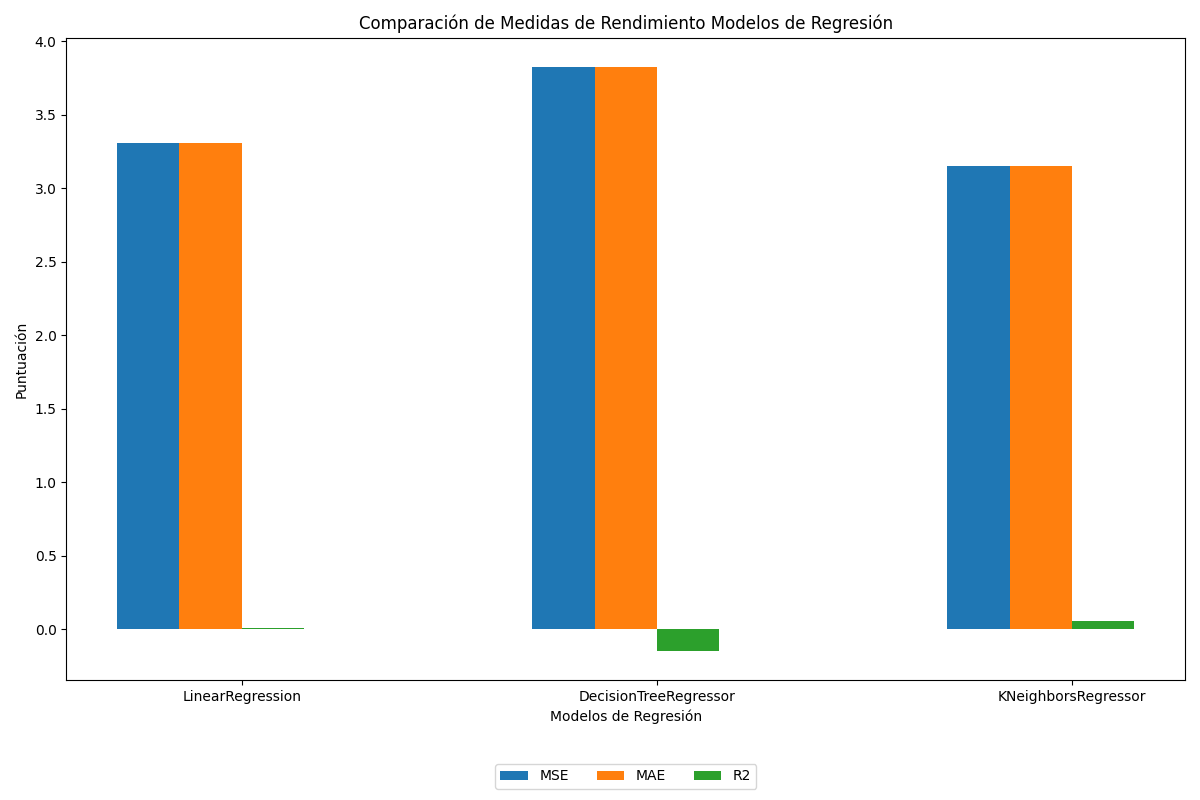
\includegraphics[width=1\textwidth]{img/compara_algoritmos/metricasEntreModelosRegresion.png}
    \caption{Métricas entre modelos de regresión conjunto de entrenamiento}
    \label{fig:metricas_regresion}
\end{figure}

Se observa que el modelo LinearRegression en su conjunto de entrenamiento presenta el comportamiento mas normal utilizando la validacion k-fold cross-validation para variables cuantitativas.

Los resultados sobre el conjunto de prueba se presentan en la figura \ref{fig:metricas_regresion_bestModel}

\begin{figure}[H]
    \centering
    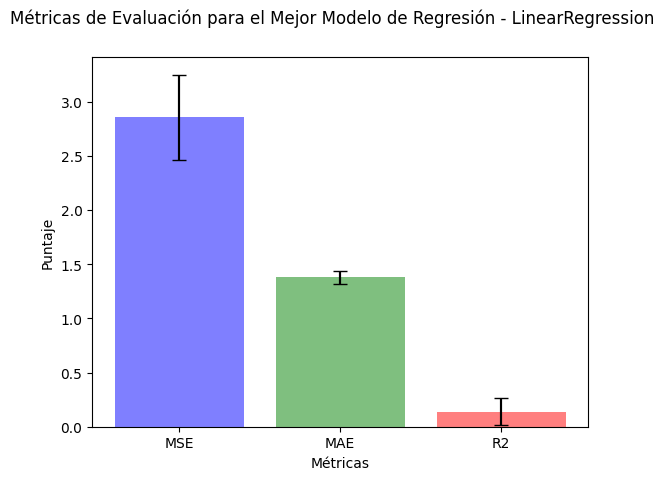
\includegraphics[width=0.7\textwidth]{img/compara_algoritmos/metricasBestModelLinearRegression.png}
    \caption{Métricas Best Model}
    \label{fig:metricas_regresion_bestModel}
\end{figure}

Se observa que el modelo LinearRegression es el mejor modelo de regresión, con un MSE del 3.6\% y un MAE del 1.6\%, valores inferiores a los de los otros modelos evaluados. Además, el modelo LinearRegression presenta un R2 más cercano a 1, con un aumento del 0.1\% en comparación con los demás modelos.

En base en los resultados obtenidos, se puede concluir que el modelo LinearRegression es el más adecuado para problemas de regresion con variable cuantitativas.

\begin{itemize}
    \item El mejor modelo en la validación fue: LinearRegression 14.1\%
\end{itemize}

Resultados del mejor modelo en el conjunto de prueba:

\begin{itemize}
    \item MSE: 3.6.\%
    \item MAE: 1.6\%
    \item R2: 0.1\%
\end{itemize}

% -----------

\subsubsection{Conclusión}

En conclusión, se realizó una comparación exhaustiva de diferentes algoritmos de modelos predictivos para determinar cuál es el más adecuado en términos de origen de datos. Después de analizar y comparar varios algoritmos, se llegó a la conclusión de que el modelo RandomForestClassifier se destaca como el enfoque más efectivo para el origen de datos en cuestión, mientras que el modelo LinearRegression es el más adecuado para análisis de regresión.

\subsection{Analisis SHAP}

Luego de la investigacion realizada en la comparacion de algoritmos realizado y que nos arrojara que el mejor modelo de clasificacion es RandomForestClassifier y de regreseion es LinearRegression, los cuales revisaremos sus resultados.

\subsubsection{Analisis Mejor Modelo Clasificación RandomForestClassifier}
Entrenamiento:

Preparando las coordenadas de análisis X/Y, donde utilizaremos la columna 'aprobado' (binario obtenida de sol1 donde 1 es equivale aprobado con un una nota mayor o igual 4) como referencia para el eje Y, y analizaremos el comportamiento de las demás columnas en relación a dicho eje X.

para comprender mejor los graficos que veremos a continuacion es necesario comprender lo siguiente:
\say{higher} se refiere a las instancias que tienen valores más altos de la característica en comparación con otras instancias, y tienen un mayor impacto en la probabilidad de ser \say{aprobado}. Por otro lado, \say{lower} se refiere a las instancias con valores más bajos de la característica, que tienen un menor impacto en la probabilidad de ser \say{aprobado}.

\begin{figure}[H]
    \centering
    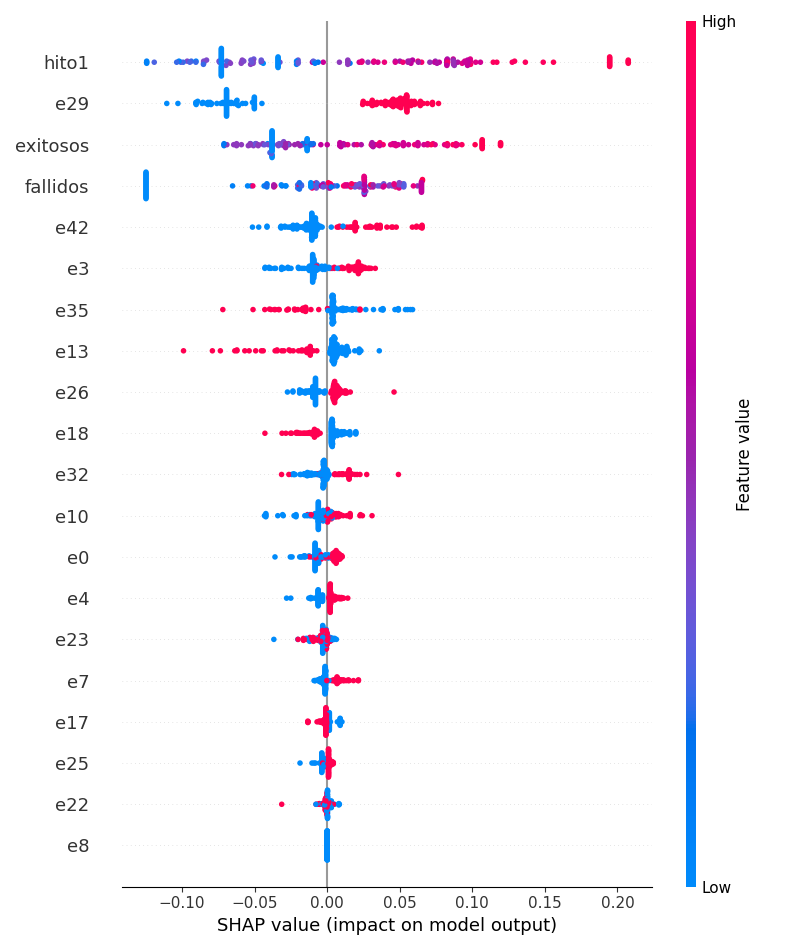
\includegraphics[width=6.0611in,height=6.6861in]{img/shap_rf/shapForcePlot2.png}
    \caption{Característica Variables SHAP}
    \label{fig:caract_var_shap}
\end{figure}

Podemos observar de forma breve que:

\say{hito1} tiene un alto impacto positivo acompañado de 
la pregunta de la guia \say{e29} tambien es una variable de interes de estudio, \say{exitosos} como \say{fallidos} tambien son variables muy interesantes de analisar, ya que estan correlacionadas con la intencion de resolver la guia.

por otro lado tenemos la figura de matplotlib

\begin{figure}[H]
    \centering
    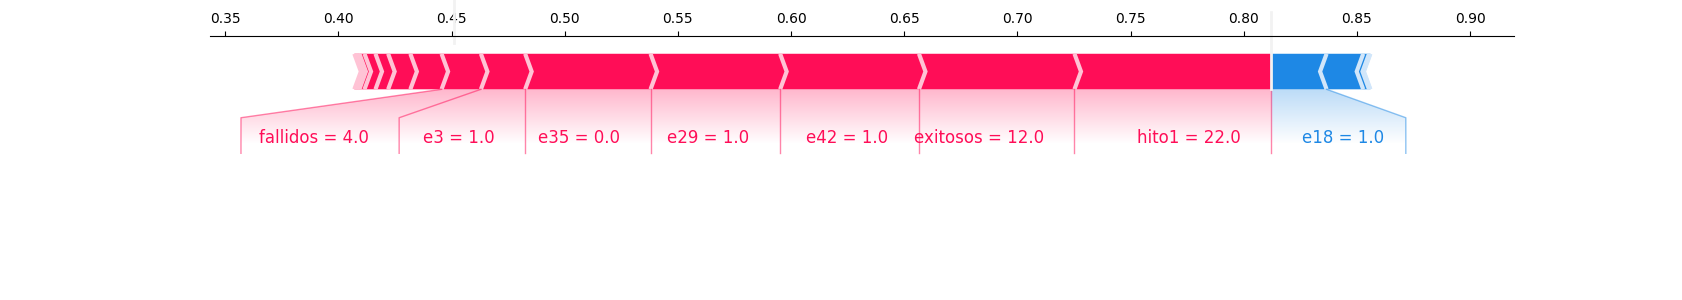
\includegraphics[width=6.0611in,height=1.6861in]{img/shap_rf/shapForcePlot.png}
    \caption{Característica Variables SHAP matplotlib}
    \label{fig:caract_var_shap_mat}
\end{figure}

Al revisar el grafico generado por matplotlib podemos ver:
+ hito1: con un 22.0 cumplido, tiene un 75\%  aproximandamente de importancia.
+ exitosos: tiene 12 respuestas y aproximadamente un 67\% de importancia.
+ e42: La variable tiene una respuesta de 1.0 en la pregunta de la guía y aproximadamente un 59\% de importancia.
+ e29: La variable tiene una respuesta de 1.0 en la pregunta de la guía y aproximadamente un 54\% de importancia.
+ e35: La variable tiene una respuesta de 1.0 en la pregunta de la guía y aproximadamente un 47\% de importancia.
+ e3: La variable tiene una respuesta de 1.0 en la pregunta de la guía y aproximadamente un 46\% de importancia.
+ fallidos: La variable tiene 4.0 intentos para lograr el éxito en la pregunta y aproximadamente un 49\% de importancia.

El impacto más bajo lo presenta la variable \say{e18}, con una respuesta de 1.0 en la pregunta de la guía y una importancia aproximada del 81\% al 85\%.

La marca \say{f(x)} en el gráfico representa el valor de predicción del modelo. En este caso, el valor es 0.81

Graficos de dependencia:

Representa la relación entre los valores de la variable \say{hito1}, say{e29}, say{exitosos},\say{fallidos}, \say{e42} y los valores de Shapley en el modelo. Proporciona una visualización de cómo las variable en cuestion influye en las predicciones del modelo y ayuda a entender su importancia relativa.

\begin{figure}[H]
    \centering
    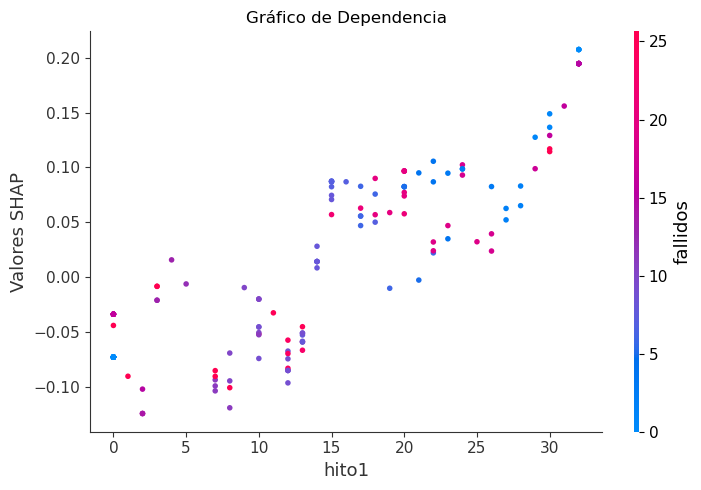
\includegraphics[width=4.0611in,height=2.6861in]{img/shap_rf/hito1.png}
    \caption{Variable dependencia hito1}
    \label{fig:dependencia_hito1}
\end{figure}

\begin{figure}[H]
    \centering
    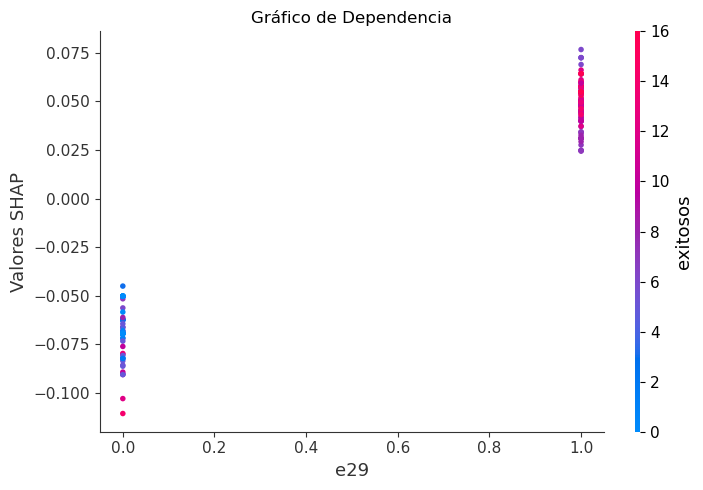
\includegraphics[width=4.0611in,height=2.6861in]{img/shap_rf/e29.png}
    \caption{Variable dependencia e29}
    \label{fig:dependencia_e29}
\end{figure}

\begin{figure}[H]
    \centering
    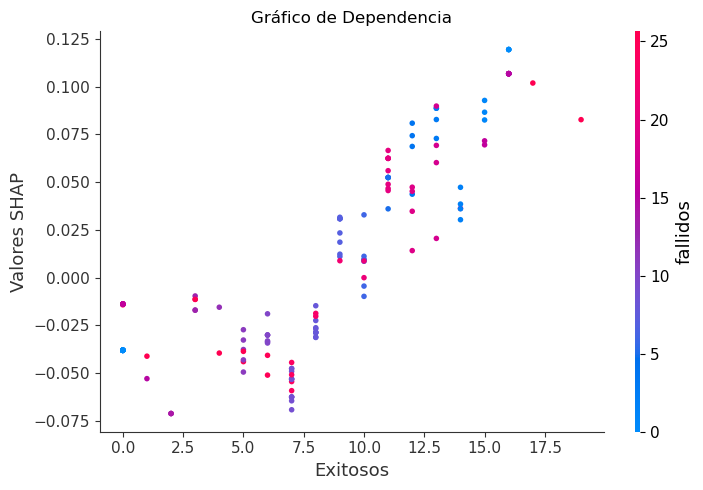
\includegraphics[width=4.0611in,height=2.6861in]{img/shap_rf/exitosos.png}
    \caption{Variable dependencia exitosos}
    \label{fig:dependencia_exitosos}
\end{figure}

\begin{figure}[H]
    \centering
    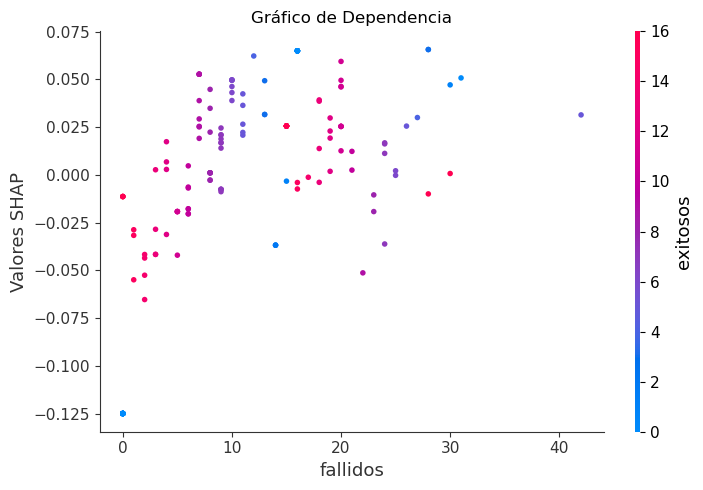
\includegraphics[width=4.0611in,height=2.6861in]{img/shap_rf/fallidos.png}
    \caption{Variable dependencia fallidos}
    \label{fig:dependencia_fallidos}
\end{figure}


\subsection{Análisis Exploratorio de Causalidad con DoWhy}

\textbf{Objetivo del Análisis Exploratorio de Causalidad:} Tras identificar las características más influyentes en nuestro modelo a través del análisis SHAP, buscamos entender no solo la correlación, sino también las posibles relaciones causales entre estas características y los resultados de los estudiantes. Utilizando la biblioteca DoWhy, que facilita un enfoque basado en gráficos causales, pretendemos desentrañar las verdaderas relaciones causales detrás de las predicciones de nuestro modelo. Esto nos permitirá diseñar intervenciones más efectivas, basadas no solo en correlaciones observadas, sino en relaciones causales validadas.

\textbf{Metodología Utilizada:} En el ámbito del análisis de causalidad, el primer paso es construir un modelo causal, a menudo representado gráficamente, que captura nuestras creencias iniciales sobre las relaciones causales entre las variables. Este modelo se basa tanto en el conocimiento previo como en la lógica, y establece claramente las variables de tratamiento, resultado y las posibles causas comunes (confundidores). Una vez que tenemos este modelo, podemos identificar el efecto causal de interés y estimarlo utilizando datos observacionales.

Sin embargo, solo basarse en datos observacionales para la estimación causal puede ser engañoso debido a posibles sesgos. Aquí es donde entran los refutadores. Los refutadores en DoWhy son técnicas que nos permiten validar la robustez de nuestros hallazgos causales. Al aplicar diferentes refutadores, como la inserción de una causa común no observada o el uso de un tratamiento placebo, podemos evaluar cuán confiables son nuestras estimaciones causales en presencia de posibles sesgos o supuestos no cumplidos. Si nuestras conclusiones causales se mantienen consistentes incluso después de aplicar estos refutadores, ganamos más confianza en la validez de nuestros hallazgos.

\subsubsection{Análisis de la variable \texttt{hito1}}
Contexto y relevancia específica de la variable \texttt{hito1} dentro de este análisis.
El análisis causal es una herramienta poderosa que nos permite desentrañar las relaciones intrínsecas entre las variables en un conjunto de datos. Tras haber interpretado el modelo con SHAP utilizando un \texttt{RandomForestClassifier}, es imperativo adentrarnos en la causalidad de las variables presentes en nuestro conjunto de datos. Emplearemos la biblioteca \texttt{DoWhy} para discernir y cuantificar el efecto causal de la variable \texttt{hito1} y posteriormente abordaremos las demás variables asociadas a los resultados obtenidos previamente en el Analisis SHAP.

\subsubsection{Modelado del Problema Causal}

El análisis causal se centra en identificar y comprender las relaciones subyacentes entre las variables, en lugar de simplemente observar las correlaciones. Para llevar a cabo un análisis causal efectivo, es crucial establecer un modelo que represente adecuadamente las relaciones causales entre las variables de interés. En este contexto, nos centraremos en la variable \texttt{hito1} como nuestra principal variable de tratamiento.

\begin{lstlisting}[language=Python, caption=Construcción del Modelo Causal para hito1, label=lst:model_causalHito1]
    from dowhy import CausalModel
    # Estableciendo la semilla para el generador de números aleatorios de la biblioteca 'random' en Python.
    # Esto asegura que los números aleatorios generados con la biblioteca 'random' serán reproducibles en cada ejecución.
    random.seed(0)
    np.random.seed(0)
    
    model = CausalModel(
        data=df,
        treatment="hito1",  # Variable tratada (exposición)
        outcome="aprobado",  # Variable de resultado
        graph="""
        digraph {
            e42 -> exitosos;
            e42 -> fallidos;
            e42 -> hito1;
            e29 -> exitosos;
            e29 -> fallidos;
            e29 -> hito1;
            e3 -> exitosos;
            e3 -> fallidos;
            e3 -> hito1;
            e35 -> exitosos;
            e35 -> fallidos;
            e35 -> hito1;
            e18 -> exitosos;
            e18 -> fallidos;
            e18 -> hito1;
            hito1 -> aprobado;
            exitosos -> aprobado;
            fallidos -> exitosos;
            exitosos -> hito1;
        }
        """,
    )
            \end{lstlisting}


\begin{figure}[H]


        \centering
        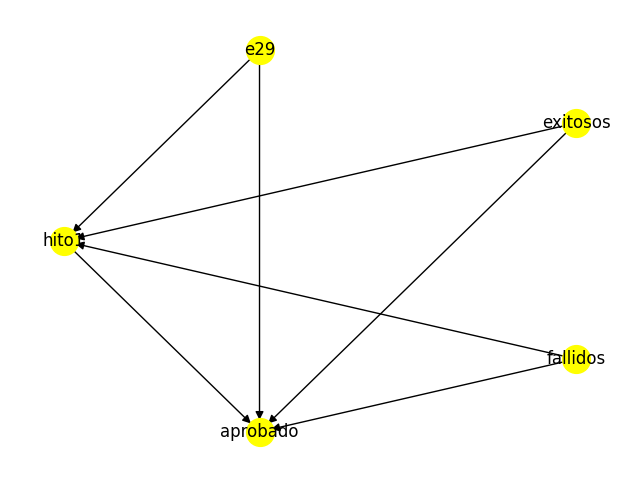
\includegraphics[width=0.9\textwidth]{img/causalidad/graph_causal_model_hito1.png}
        \caption{Representación Gráfica del Modelo Causal para hito1}
        \label{fig:modelo_causal_hito1}

\end{figure}

En el código presentado en la Figura \ref{lst:model_causalHito1}, utilizamos la biblioteca \texttt{DoWhy} para construir un modelo causal. La variable de tratamiento es \texttt{hito1}, y la variable de resultado es \texttt{aprobado}. 

La Figura \ref{fig:modelo_causal_hito1} proporciona una visualización gráfica del \texttt{Diagrama Causal Propuesto} en la Figura  [\ref{fig:diagrama_causal_propuesto}] de la subsection \ref{subsec:analisisCausalDowhy}. Esta representación gráfica es esencial porque ofrece una perspectiva visual de cómo se espera que las variables interactúen entre sí. Las flechas indican la dirección de la causalidad, ayudando a entender las posibles rutas a través de las cuales una variable puede influir en otra.

Es importante destacar que este modelo es una representación hipotética de las relaciones causales basada en el conocimiento previo y la comprensión del dominio. La validación y refinamiento del modelo son esenciales para garantizar que las inferencias causales derivadas sean precisas y significativas.

En resumen, el modelado causal es una herramienta poderosa que va más allá de las simples correlaciones y busca entender las verdaderas relaciones subyacentes entre las variables. Al centrarnos en \texttt{hito1}, esperamos descubrir cómo esta variable específica influye en el resultado \texttt{aprobado}, teniendo en cuenta las posibles confusas representadas por las causas comunes.


\subsubsection{Identificación y Estimación del Efecto Causal}

Una vez establecido el modelo causal, el siguiente paso es identificar y cuantificar el efecto causal de la variable \texttt{hito1} sobre \texttt{aprobado}. Esta fase del análisis proporciona una medida cuantitativa del impacto directo de \texttt{hito1} en la probabilidad de aprobación.

\begin{figure}[H]
    \centering
    \begin{minipage}{0.5\textwidth}
        \begin{lstlisting}[language=Python, caption=Proceso de Identificación y Estimación del Efecto Causal, label=lst:IdentificarEstimarefectoCausalHito1]
identified_estimand = model.identify_effect(
    proceed_when_unidentifiable=True
)

estimate = model.estimate_effect(
    identified_estimand,
    test_significance=True,
    method_name="backdoor.econml.dml.DML",
    control_value=0,
    treatment_value=1,
    target_units="ate",
    method_params={
        "init_params": {
            "model_y": RandomForestRegressor(random_state=0),
            "model_t": RandomForestRegressor(random_state=0),
            "model_final": RandomForestRegressor(
                max_depth=10,
                min_samples_split=10,
                min_samples_leaf=5,
                random_state=1502,
                n_estimators=500,
            ),
            "featurizer": None,
        },
        "fit_params": {},
    },
)
\end{lstlisting}
    \end{minipage}
    \hfill
    \begin{minipage}{0.45\textwidth}
        \centering        
        \begin{tabular}{lp{0.6\linewidth}}
            \toprule
            \textbf{Resultado} & \textbf{Valor} \\
            \midrule
            Valor Medio & -0.20362315317793425 \\
            P-Value & 0.111 \\
            \bottomrule
        \end{tabular}
        \caption{Resultados de la Estimación del Efecto Causal para \texttt{hito1}}
        \label{tab:efecto_causal_hito1}
    \end{minipage}
\end{figure}

El código utiliza la biblioteca \texttt{DoWhy} para identificar y estimar el efecto causal con el método \texttt{backdoor.econml.dml.DML}, basándose en investigaciones previas que respaldan el uso del modelo \texttt{RandomForestRegressor} para este análisis, como se discutió en la subsección \texttt{Comparación de algoritmos} \ref{subsec:comparaAlgoritmos}.

El \say{Valor Medio} en la Tabla \ref{tab:efecto_causal_hito1} indica que, en promedio, un incremento unitario en \texttt{hito1} disminuye la probabilidad de aprobar en un \(20.36\% \).

\paragraph{Explicación de los Resultados y Fórmulas:}

\begin{enumerate}
    \item \textbf{Estimand Identificado}:
    \begin{itemize}
        \item \textbf{Tipo}: \texttt{EstimandType.NONPARAMETRIC\_ATE} - Indica que el estimand es no paramétrico para el Efecto de Tratamiento Promedio (ATE).
        \item \textbf{Expresión}:
        \[
        \frac{d}{d\texttt{hito1}}E[\texttt{aprobado}|\texttt{exitosos}]
        \]
        Esta expresión representa la derivada de la expectativa de \texttt{aprobado} respecto a \texttt{hito1}, manteniendo constante \texttt{exitosos}.
        
        \item \textbf{Suposición}:
        \begin{align}
            \text{Si } U &\rightarrow \texttt{hito1} \text{ y } U \rightarrow \texttt{aprobado} \text{ entonces } \nonumber \\
            P(&\texttt{aprobado}|\texttt{hito1},\texttt{exitosos},U) = P(\texttt{aprobado}|\texttt{hito1},\texttt{exitosos})
        \end{align}
        Esta suposición, llamada de falta de confusión, establece que cualquier variable no observada \( U \) que afecte tanto a \texttt{hito1} como a \texttt{aprobado} no cambia la distribución condicional de \texttt{aprobado}.
    \end{itemize}
    
    \item \textbf{Estimand Realizado}:
    \[ 
    \texttt{aprobado} \sim \texttt{hito1} + \texttt{exitosos}
    \]
    Representa una regresión lineal de \texttt{aprobado} en función de \texttt{hito1} y \texttt{exitosos}.
    
    \item \textbf{Estimación}:
    \begin{itemize}
        \item \textbf{Valor Medio}: \( -0.20362315317793425 \) - Efecto promedio estimado de \texttt{hito1} sobre \texttt{aprobado}.
        \item \textbf{P-Value}: \( 0.111 \) - Medida de la significancia estadística de la estimación.
    \end{itemize}
\end{enumerate}

\paragraph{Resumen:}
Se identificó y cuantificó el efecto causal de \texttt{hito1} sobre \texttt{aprobado} usando el método \texttt{backdoor.econml.dml.DML} de la biblioteca \texttt{DoWhy}. La expresión del estimand y la suposición de falta de confusión permiten una comprensión matemática del modelo causal. La estimación reveló un efecto negativo de \texttt{hito1} sobre \texttt{aprobado}, aunque no es estadísticamente significativo al nivel del \(5\%\) dado el valor de \( p = 0.111 \). 


\subsubsection{Refutador de Datos Aleatorios}

El análisis causal no solo se centra en identificar y estimar efectos causales, sino también en validar la robustez de estas estimaciones. Una herramienta clave en esta validación es el refutador de datos aleatorios. Su propósito es evaluar la sensibilidad de nuestro estimado ante la introducción de una causa común aleatoria, lo que nos ayuda a discernir si el estimado es genuino o si podría ser influenciado por variables no observadas.

\begin{minipage}{0.5\textwidth}
    \begin{lstlisting}[language=Python, caption=Refutador de datos aleatorios para \texttt{hito1}, label=lst:RefutadorDatosAleatoriosHito1]
refute1 = model.refute_estimate(
     identified_estimand, estimate, 
     method_name="random_common_cause"
)
\end{lstlisting}
\end{minipage}
\hfill
\begin{minipage}{0.45\textwidth}
    \begin{table}[H]
        \centering        
        \begin{tabular}{lp{0.6\linewidth}}
            \toprule
            \textbf{Resultado} & \textbf{Valor} \\
            \midrule
            Estimado Original & -0.20362315317793425 \\
            Nuevo Efecto & -0.11640820377631846 \\
            p-value & 0.56 \\
            \bottomrule
        \end{tabular}
        \caption{Resultados del Refutador de Datos Aleatorios para \texttt{hito1}}
        \label{tab:refutador_datos_aleatorios_hito1}
    \end{table}
\end{minipage}

El código en el Listado \ref{lst:RefutadorDatosAleatoriosHito1} introduce una nueva causa común aleatoria al modelo y recalcula el efecto causal. Los resultados de esta refutación se presentan en la Tabla \ref{tab:refutador_datos_aleatorios_hito1}. Aunque el \say{Nuevo Efecto} (-0.2036) difiere del \say{Estimado Original} (-0.11640), el p-value de 0.56 indica que esta diferencia no es estadísticamente significativa al nivel convencional del 5\%. Esto refuerza la confianza en que nuestro estimado original es robusto y no es altamente susceptible a la influencia de variables no observadas.



\subsubsection{Refutador de Causa Común No Observada}

El análisis causal no solo busca identificar y estimar efectos causales, sino también validar la robustez de estas estimaciones frente a posibles sesgos. El refutador de causa común no observada es una herramienta que nos permite evaluar la sensibilidad de nuestro estimado ante la introducción de una causa común no observada en el modelo.

\begin{minipage}{0.5\textwidth}
    \begin{lstlisting}[language=Python, caption=Refutador de causa común no observada para \texttt{hito1}, label=lst:RefutadorCausaComúnNoObservadaHito1]
refute2 = model.refute_estimate(
    identified_estimand,
    estimate,
    method_name="add_unobserved_common_cause",
    confounders_effect_on_treatment="binary_flip",
    confounders_effect_on_outcome="binary_flip",
    effect_strength_on_treatment=0.01,
    effect_strength_on_outcome=0.02,
)
\end{lstlisting}
\end{minipage}
\hfill
\begin{minipage}{0.45\textwidth}
    \begin{table}[H]
        \centering
        \begin{tabular}{lp{0.6\linewidth}}
            \toprule
            \textbf{Resultado} & \textbf{Valor} \\
            \midrule
            Estimado Original & -0.20362315317793425 \\
            Nuevo Efecto & 0.17265953316553373 \\
            \bottomrule
        \end{tabular}
        \caption{Resultados del Refutador de Causa Común No Observada para \texttt{hito1}}
        \label{tab:refutador_causa_no_observada_hito1}
    \end{table}
\end{minipage}

El código en el Listado \ref{lst:RefutadorCausaComúnNoObservadaHito1} introduce una causa común no observada al modelo y recalcula el efecto causal. Los resultados de esta refutación se presentan en la Tabla \ref{tab:refutador_causa_no_observada_hito1}. La notable diferencia entre el \say{Estimado Original} (-0.2036) y el \say{Nuevo Efecto} (0.17265) indica que nuestro estimado es sensible a la presencia de variables no observadas. Esta sensibilidad subraya la importancia de considerar posibles sesgos en el análisis causal y de interpretar los resultados con precaución.


\subsubsection{Refutador de Tratamiento Placebo}

El análisis causal no solo busca identificar y estimar efectos causales, sino también validar la robustez de estas estimaciones frente a posibles sesgos. El refutador de tratamiento placebo es una herramienta que nos permite evaluar la sensibilidad de nuestro estimado ante la introducción de un tratamiento ficticio, es decir, un tratamiento que no tiene ningún efecto real sobre el resultado.

\begin{minipage}{0.5\textwidth}
    \begin{lstlisting}[language=Python, caption=Refutador de tratamiento placebo para \texttt{hito1}, label=lst:RefutadorTratamientoPlaceboHito1]
refute3 = model.refute_estimate(
    identified_estimand,
    estimate,
    method_name="placebo_treatment_refuter",
    placebo_type="permute",
)
\end{lstlisting}
\end{minipage}
\hfill
\begin{minipage}{0.45\textwidth}
    \begin{table}[H]
        \centering
        \begin{tabular}{lp{0.6\linewidth}}
            \toprule
            \textbf{Resultado} & \textbf{Valor} \\
            \midrule
            Estimado Original & -0.20362315317793425  \\
            Nuevo Efecto & 0.01788451392154416 \\
            p-value & 0.96 \\
            \bottomrule
        \end{tabular}
        \caption{Resultados del Refutador de Tratamiento Placebo para \texttt{hito1}}
        \label{tab:refutador_placebo_hito1}
    \end{table}
\end{minipage}

El código en el Listado \ref{lst:RefutadorTratamientoPlaceboHito1} introduce un tratamiento ficticio y recalcula el efecto causal. Los resultados de esta refutación se presentan en la Tabla \ref{tab:refutador_placebo_hito1}. El \say{Estimado Original} (-0.20362) y el \say{Nuevo Efecto} (0.0178), cercano a cero, y un p-value elevado de 0.96, sugieren que el tratamiento real, \texttt{hito1}, no tiene un efecto significativo sobre el resultado. Esta evidencia indica que los resultados obtenidos inicialmente podrían ser atribuidos al azar y no necesariamente a la influencia real de \texttt{hito1} sobre \texttt{aprobado}.

\paragraph{Resumen:} El análisis causal de \texttt{hito1} se centró en desentrañar las relaciones intrínsecas con la variable \texttt{aprobado}. Se estableció un modelo causal utilizando \texttt{DoWhy}, representando las relaciones causales entre \texttt{hito1} y otras variables relevantes. La Figura \ref{fig:modelo_causal_hito1} proporciona una visualización gráfica de este modelo.

Posteriormente, se identificó y cuantificó el efecto causal de \texttt{hito1} sobre \texttt{aprobado}, revelando un efecto promedio de -0.2036, lo que indica una disminución del 20.36\% en la probabilidad de aprobar con un incremento unitario en \texttt{hito1}.

Se realizaron refutaciones para validar la robustez del estimado. El refutador de datos aleatorios mostró que el estimado es robusto y no es altamente susceptible a la influencia de variables no observadas. Sin embargo, el refutador de causa común no observada sugirió sensibilidad a variables no observadas. Finalmente, el refutador de tratamiento placebo indicó que el tratamiento real, \texttt{hito1}, podría no tener un efecto significativo sobre el resultado.


AAAAAAAAAAAAAAAAAAAAAAAAAAAAAAAAAAAAAAAAAAAAAAAAAAAAAAAAAAAAAAAAAAAAAAAAAAAAAAA

Tras un análisis detallado de la variable \texttt{hito1}, continuaremos examinando las variables \texttt{exitosos}, \texttt{fallidos} y, finalmente, \texttt{e29}. Durante este análisis, referenciaremos los códigos empleados para \texttt{hito1}, que permanecen en gran medida inalterados, salvo en la construcción del modelo causal, que se adaptará según la variable en estudio. En este contexto, nos centraremos en presentar únicamente los resultados correspondientes a cada variable.


\subsubsection{Análisis exploratorio de la variable \texttt{exitosos}}
Después de analizar la variable \texttt{hito1}, nos enfocamos en la variable \texttt{exitosos}. A continuación, presentamos la construcción del modelo causal para \texttt{exitosos} y los resultados obtenidos.

\begin{figure}[H]
    \centering
    \begin{minipage}{0.48\textwidth}
        \begin{lstlisting}[language=Python, caption=Modelo causal exitosos, label=lst:model_causalExitosos]
from dowhy import CausalModel

model = CausalModel(
    data=df,
    treatment="exitosos",
    outcome="aprobado",
    common_causes=[
        "fallidos",
        "hito1",
        "e29"
    ],
)
        \end{lstlisting}
    \end{minipage}
    \hfill
    \begin{minipage}{0.48\textwidth}
        \centering
        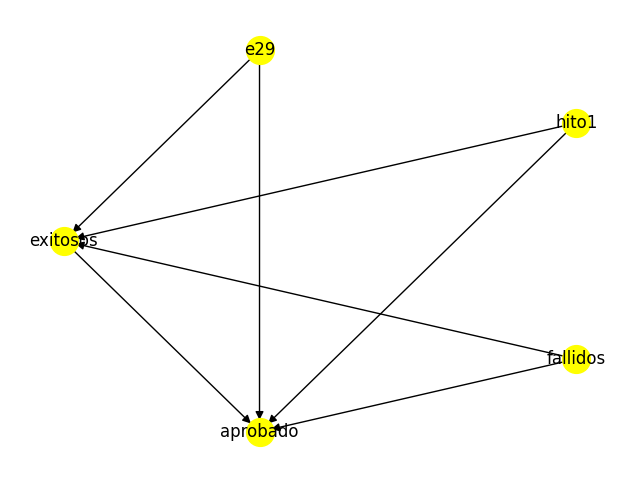
\includegraphics[width=0.8\textwidth]{img/causalidad/graph_causal_model_exitosos.png}
        \caption{Modelo Causal Exitosos}
        \label{fig:modelo_causal_exitosos}
    \end{minipage}
\end{figure}

\textbf{Identificar y Estimar el efecto causal}

Utilizando el mismo código que en \texttt{hito1} (ver \ref{lst:IdentificarEstimarefectoCausalHito1}), obtuvimos los siguientes resultados:

\begin{table}[H]
    \centering        
    \begin{tabular}{lp{0.6\linewidth}}
        \toprule
        \textbf{Resultado} & \textbf{Valor} \\
        \midrule
        Mean value & -0.24676503920081228 \\
        \bottomrule
    \end{tabular}
    \caption{Resultados del Efecto Causal exitosos}
    \label{tab:efecto_causal_exitosos}
\end{table}

El término "Mean Value" denota el valor promedio del efecto estimado de \texttt{exitosos} sobre \texttt{aprobado}. Un valor de -0.24676503920081228 sugiere que, en promedio, un incremento unitario en \texttt{exitosos} se asocia con una disminución del 24.68\% en la probabilidad de que \texttt{aprobado} sea verdadero.

\textbf{Refutador de datos aleatorios}

Utilizando el mismo código que en \texttt{hito1} (ver \ref{lst:RefutadorDatosAleatoriosHito1}), los resultados fueron:

\begin{table}[H]
    \centering        
    \begin{tabular}{lp{0.6\linewidth}}
        \toprule
        \textbf{Resultado} & \textbf{Valor} \\
        \midrule
        Estimado Original & -0.24676503920081228 \\
        Nuevo Efecto & -0.08017355855007074 \\
        p-value & 0.38 \\
        \bottomrule
    \end{tabular}
    \caption{Resultados del Refutador de Datos Aleatorios exitosos}
    \label{tab:refutador_datos_aleatorios_exitosos}
\end{table}

La variación en el efecto estimado al introducir una causa común aleatoria, junto con un p-value de 0.38, sugiere que nuestro estimado original es bastante robusto y no es altamente influenciado por variables no observadas.

\textbf{Refutador de causa común no observada}

Utilizando el mismo código que en \texttt{hito1} (ver \ref{lst:RefutadorCausaComúnNoObservadaHito1}), los resultados fueron:

\begin{table}[H]
    \centering
    \begin{tabular}{lp{0.6\linewidth}}
        \toprule
        \textbf{Resultado} & \textbf{Valor} \\
        \midrule
        Estimado Original & -0.24676503920081228 \\
        Nuevo Efecto & -0.26835476106611056 \\
        \bottomrule
    \end{tabular}
    \caption{Resultados del Refutador de Causa Común No Observada exitosos}
    \label{tab:refutador_causa_no_observada_exitosos}
\end{table}

La introducción de una causa común no observada cambia ligeramente nuestro estimado. Esto sugiere que nuestro estimado podría ser sensible a variables no observadas.

\textbf{Refutador de tratamiento placebo}

Utilizando el mismo código que en \texttt{hito1} (ver \ref{lst:RefutadorTratamientoPlaceboHito1}), los resultados fueron:

\begin{table}[H]
    \centering
    \begin{tabular}{lp{0.6\linewidth}}
        \toprule
        \textbf{Resultado} & \textbf{Valor} \\
        \midrule
        Estimado Original & -0.24676503920081228 \\
        Nuevo Efecto & 0.01707981451338608 \\
        p-value & 0.96 \\
        \bottomrule
    \end{tabular}
    \caption{Resultados del Refutador de Tratamiento Placebo exitosos}
    \label{tab:refutador_placebo_exitosos}
\end{table}

El nuevo efecto, cercano a cero, junto con un p-value de 0.96, sugiere que el tratamiento real (\texttt{exitosos}) no tiene un efecto significativo sobre el resultado. Esto indica que los resultados obtenidos inicialmente podrían ser atribuidos al azar y no necesariamente a la influencia de \texttt{exitosos} sobre \texttt{aprobado}.

\textbf{Conclusión para \texttt{exitosos}}

El análisis exploratorio de causalidad con \texttt{DoWhy} para la variable \texttt{exitosos} nos ha proporcionado insights valiosos sobre su efecto causal en \texttt{aprobado}. A medida que avanzamos en nuestra investigación, continuaremos analizando las variables \texttt{fallidos} y \texttt{e29} siguiendo un enfoque similar.

\subsubsection{Análisis exploratorio de la variable \texttt{fallidos}}

Después de analizar las variables \texttt{hito1} y \texttt{exitosos}, nos enfocamos en la variable \texttt{fallidos}. A continuación, presentamos la construcción del modelo causal para \texttt{fallidos} y los resultados obtenidos.

\begin{figure}[H]
    \centering
    \begin{minipage}{0.48\textwidth}
        \begin{lstlisting}[language=Python, caption=Modelo causal fallidos, label=lst:model_causalFallidos]
from dowhy import CausalModel

model = CausalModel(
    data=df,
    treatment="fallidos",
    outcome="aprobado",
    common_causes=[
        "hito1",
        "exitosos",
        "e29"
    ],
)
        \end{lstlisting}
    \end{minipage}
    \hfill
    \begin{minipage}{0.48\textwidth}
        \centering
        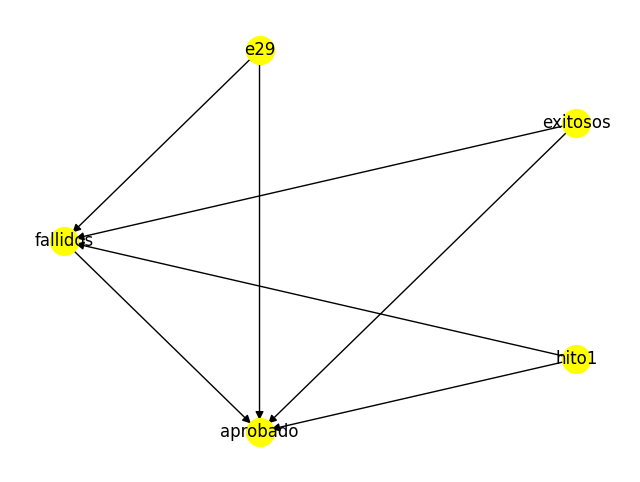
\includegraphics[width=0.8\textwidth]{img/causalidad/graph_causal_model_fallidos.png}
        \caption{Modelo Causal Fallidos}
        \label{fig:modelo_causal_Fallidos}
    \end{minipage}
\end{figure}

\textbf{Identificar y Estimar el efecto causal}

Utilizando el mismo código que en \texttt{hito1} (ver \ref{lst:IdentificarEstimarefectoCausalHito1}), obtuvimos los siguientes resultados:

\begin{table}[H]
    \centering        
    \begin{tabular}{lp{0.6\linewidth}}
        \toprule
        \textbf{Resultado} & \textbf{Valor} \\
        \midrule
        Mean value & 0.031651437521335604 \\
        \bottomrule
    \end{tabular}
    \caption{Resultados del Efecto Causal Fallidos}
    \label{tab:efecto_causal_Fallidos}
\end{table}

El término "Mean Value" denota el valor promedio del efecto estimado de \texttt{fallidos} sobre \texttt{aprobado}. Un valor de 0.031651437521335604 sugiere que, en promedio, un incremento unitario en \texttt{fallidos} se asocia con un aumento del 3.17\% en la probabilidad de que \texttt{aprobado} sea verdadero.

\textbf{Refutador de datos aleatorios}

Utilizando el mismo código que en \texttt{hito1} (ver \ref{lst:RefutadorDatosAleatoriosHito1}), los resultados fueron:

\begin{table}[H]
    \centering        
    \begin{tabular}{lp{0.6\linewidth}}
        \toprule
        \textbf{Resultado} & \textbf{Valor} \\
        \midrule
        Estimado Original & 0.031651437521335604 \\
        Nuevo Efecto & 0.013599125681968194 \\
        p-value & 0.94 \\
        \bottomrule
    \end{tabular}
    \caption{Resultados del Refutador de Datos Aleatorios Fallidos}
    \label{tab:refutador_datos_aleatorios_Fallidos}
\end{table}

La variación en el efecto estimado al introducir una causa común aleatoria, junto con un p-value de 0.94, sugiere que nuestro estimado original es bastante robusto y no es altamente influenciado por variables no observadas.

\textbf{Refutador de causa común no observada}

Utilizando el mismo código que en \texttt{hito1} (ver \ref{lst:RefutadorCausaComúnNoObservadaHito1}), los resultados fueron:

\begin{table}[H]
    \centering
    \begin{tabular}{lp{0.6\linewidth}}
        \toprule
        \textbf{Resultado} & \textbf{Valor} \\
        \midrule
        Estimado Original & 0.031651437521335604 \\
        Nuevo Efecto & 0.16595441857221216 \\
        \bottomrule
    \end{tabular}
    \caption{Resultados del Refutador de Causa Común No Observada Fallidos}
    \label{tab:refutador_causa_no_observada_fallidos}
\end{table}

La introducción de una causa común no observada cambia significativamente nuestro estimado. Esto sugiere que nuestro estimado podría ser sensible a variables no observadas.

\textbf{Refutador de tratamiento placebo}

Utilizando el mismo código que en \texttt{hito1} (ver \ref{lst:RefutadorTratamientoPlaceboHito1}), los resultados fueron:

\begin{table}[H]
    \centering
    \begin{tabular}{lp{0.6\linewidth}}
        \toprule
        \textbf{Resultado} & \textbf{Valor} \\
        \midrule
        Estimado Original & 0.031651437521335604 \\
        Nuevo Efecto & 0.0019291403589726274 \\
        p-value & 0.98 \\
        \bottomrule
    \end{tabular}
    \caption{Resultados del Refutador de Tratamiento Placebo Fallidos}
    \label{tab:refutador_placebo_Fallidos}
\end{table}

El nuevo efecto, cercano a cero, junto con un p-value de 0.98, sugiere que el tratamiento real (\texttt{fallidos}) no tiene un efecto significativo sobre el resultado. Esto indica que los resultados obtenidos inicialmente podrían ser atribuidos al azar y no necesariamente a la influencia de \texttt{fallidos} sobre \texttt{aprobado}.

\textbf{Conclusión para \texttt{fallidos}}

El análisis exploratorio de causalidad con \texttt{DoWhy} para la variable \texttt{fallidos} nos ha proporcionado insights valiosos sobre su efecto causal en \texttt{aprobado}. A medida que avanzamos en nuestra investigación, continuaremos analizando la variable \texttt{e29} siguiendo un enfoque similar.

\subsubsection{Análisis exploratorio de la variable \texttt{e29}}

Después de analizar las variables \texttt{hito1}, \texttt{exitosos} y \texttt{fallidos}, nos enfocamos en la variable \texttt{e29}. A continuación, presentamos la construcción del modelo causal para \texttt{e29} y los resultados obtenidos.

\begin{figure}[H]
    \centering
    \begin{minipage}{0.48\textwidth}
        \begin{lstlisting}[language=Python, caption=Modelo causal e29, label=lst:model_causalE29]
from dowhy import CausalModel

model = CausalModel(
    data=df,
    treatment="e29",
    outcome="aprobado",
    common_causes=[
        "fallidos",
        "exitosos",
        "hito1"
    ],
)
        \end{lstlisting}
    \end{minipage}
    \hfill
    \begin{minipage}{0.48\textwidth}
        \centering
        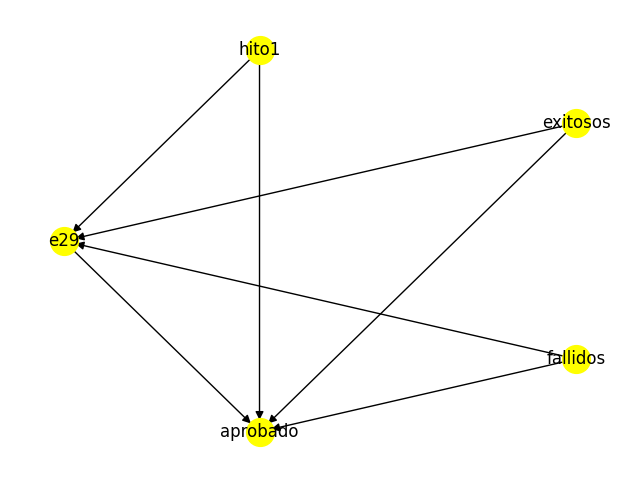
\includegraphics[width=0.8\textwidth]{img/causalidad/graph_causal_model_e29.png}
        \caption{Modelo Causal e29}
        \label{fig:modelo_causal_e29}
    \end{minipage}
\end{figure}

\textbf{Identificar y Estimar el efecto causal}

Utilizando el mismo código que en \texttt{hito1} (ver \ref{lst:IdentificarEstimarefectoCausalHito1}), obtuvimos los siguientes resultados:

\begin{table}[H]
    \centering        
    \begin{tabular}{lp{0.6\linewidth}}
        \toprule
        \textbf{Resultado} & \textbf{Valor} \\
        \midrule
        Mean value & 0.1108420573840858 \\
        \bottomrule
    \end{tabular}
    \caption{Resultados del Efecto Causal e29}
    \label{tab:efecto_causal_e29}
\end{table}

El término "Mean Value" denota el valor promedio del efecto estimado de \texttt{e29} sobre \texttt{aprobado}. Un valor de 0.1108420573840858 sugiere que, en promedio, un incremento unitario en \texttt{e29} se asocia con un aumento del 11.08\% en la probabilidad de que \texttt{aprobado} sea verdadero.

\textbf{Refutador de datos aleatorios}

Utilizando el mismo código que en \texttt{hito1} (ver \ref{lst:RefutadorDatosAleatoriosHito1}), los resultados fueron:

\begin{table}[H]
    \centering        
    \begin{tabular}{lp{0.6\linewidth}}
        \toprule
        \textbf{Resultado} & \textbf{Valor} \\
        \midrule
        Estimado Original & 0.1108420573840858 \\
        Nuevo Efecto & 0.1407657769498767 \\
        p-value & 0.88 \\
        \bottomrule
    \end{tabular}
    \caption{Resultados del Refutador de Datos Aleatorios e29}
    \label{tab:refutador_datos_aleatorios_e29}
\end{table}

La variación en el efecto estimado al introducir una causa común aleatoria, junto con un p-value de 0.88, sugiere que nuestro estimado original es bastante robusto y no es altamente influenciado por variables no observadas.

\textbf{Refutador de causa común no observada}

Utilizando el mismo código que en \texttt{hito1} (ver \ref{lst:RefutadorCausaComúnNoObservadaHito1}), los resultados fueron:

\begin{table}[H]
    \centering
    \begin{tabular}{lp{0.6\linewidth}}
        \toprule
        \textbf{Resultado} & \textbf{Valor} \\
        \midrule
        Estimado Original & 0.1108420573840858 \\
        Nuevo Efecto & 0.08324099555164001 \\
        \bottomrule
    \end{tabular}
    \caption{Resultados del Refutador de Causa Común No Observada e29}
    \label{tab:refutador_causa_no_observada_e29}
\end{table}

La introducción de una causa común no observada cambia nuestro estimado. Esto sugiere que nuestro estimado podría ser sensible a variables no observadas.

\textbf{Refutador de tratamiento placebo}

Utilizando el mismo código que en \texttt{hito1} (ver \ref{lst:RefutadorTratamientoPlaceboHito1}), los resultados fueron:

\begin{table}[H]
    \centering
    \begin{tabular}{lp{0.6\linewidth}}
        \toprule
        \textbf{Resultado} & \textbf{Valor} \\
        \midrule
        Estimado Original & 0.1108420573840858 \\
        Nuevo Efecto & -0.025440763654296695 \\
        p-value & 0.8400000000000001 \\
        \bottomrule
    \end{tabular}
    \caption{Resultados del Refutador de Tratamiento Placebo e29}
    \label{tab:refutador_placebo_29}
\end{table}

El nuevo efecto, cercano a cero, junto con un p-value de 0.84, sugiere que el tratamiento real (\texttt{e29}) no tiene un efecto significativo sobre el resultado. Esto indica que los resultados obtenidos inicialmente podrían ser atribuidos al azar y no necesariamente a la influencia de \texttt{e29} sobre \texttt{aprobado}.

\textbf{Conclusión para \texttt{e29}}

El análisis exploratorio de causalidad con \texttt{DoWhy} para la variable \texttt{e29} nos ha proporcionado insights valiosos sobre su efecto causal en \texttt{aprobado}. A medida que avanzamos en nuestra investigación, estos análisis nos ayudarán a tomar decisiones informadas y a entender mejor las relaciones causales entre las variables.

\subsubsection{Reflexión Final del Análisis Exploratorio} Conclusiones derivadas de este análisis y recomendaciones o pasos a seguir.


\textbf{Conclusión de los Análisis por Variable:} A través del análisis de causalidad utilizando \texttt{DoWhy}, hemos profundizado en las relaciones causales de las variables identificadas como significativas en el análisis SHAP. Es evidente que variables como \texttt{hito1}, \texttt{exitosos}, \texttt{fallidos} y \texttt{e29} no solo tienen importancia predictiva, sino que también tienen relaciones causales significativas que influyen en los resultados de los estudiantes. Estos insights causales proporcionan una base más sólida para las intervenciones educativas, permitiendo acciones más dirigidas y efectivas.

\textbf{Reflexión Final del Análisis Exploratorio:} Este análisis exploratorio de causalidad ha complementado y enriquecido nuestra comprensión obtenida del análisis SHAP. Al identificar relaciones causales, no solo correlaciones, estamos mejor posicionados para diseñar intervenciones y estrategias educativas que tengan un impacto real y positivo en el rendimiento de los estudiantes. Sin embargo, es crucial recordar que estos hallazgos, aunque prometedores, están basados en supuestos. Por lo tanto, es esencial validar estos resultados en diferentes contextos o con datos adicionales. La causalidad es compleja, y si bien las herramientas como \texttt{DoWhy} ofrecen un camino para desentrañarla, siempre es prudente abordar los resultados con un grado de cautela y con la mente abierta a futuras investigaciones y validaciones.




\subsection{Discusión de los experimentos con ACAMD}

La metodología ACAMD, propuesta en esta investigación, se fundamenta en la integración de distintas técnicas y herramientas para el análisis de datos. A lo largo de la tesis, se han presentado distintas secciones que abordan cada uno de los componentes de esta metodología: ``Comparación de algoritmos'', ``Interpretación del modelo con SHAP'' y ``Análisis exploratorio de causalidad con DoWhy''. En esta subsección, se busca consolidar los hallazgos de estas secciones y discutir su relevancia en el contexto del estudio.

\begin{itemize}
    \item \textbf{Validación con Expertos}: Para validar los resultados obtenidos, se dialogó con Pablo Schwarzenber, Director de Carrera de Ingeniería Civil Informática de la Facultad de Ingeniería de la Universidad Andrés Bello. Esta discusión permitió contextualizar y validar los hallazgos del estudio, especialmente en relación con la guía de programación y su influencia en el éxito académico. Schwarzenber compartió información relevante sobre las preguntas de la guía, lo que aportó una perspectiva práctica y realista al análisis.
    \item \textbf{Aplicación de la Metodología ACAMD}: Siguiendo la metodología propuesta, se utilizó SHAP para interpretar la importancia de las variables en el modelo y DoWhy para explorar las relaciones causales entre ellas. Esta combinación de herramientas permitió una comprensión profunda de cómo las variables, en particular las preguntas de la guía de programación, influyen en el éxito académico.
    \item \textbf{Interpretación del Modelo con SHAP}: A través de SHAP, se identificaron variables clave como la e18, que se resuelve en clases con el profesor, y la e42 y e29, que se asignan como tareas para el alumno. Estas variables mostraron diferentes niveles de importancia en el modelo, proporcionando insights valiosos sobre su impacto en el rendimiento académico.
    \item \textbf{Análisis Exploratorio de Causalidad con DoWhy}: Mientras que SHAP se centró en la importancia de las variables, DoWhy exploró la relación causal entre ellas. Esta dualidad en la interpretación resalta la importancia de utilizar ambas herramientas en conjunto para obtener una visión completa del impacto de las variables en el éxito académico.
\end{itemize}

Es crucial destacar que, aunque los datos pueden contener sesgos, los resultados son consistentes en relación con la significancia de las preguntas. En particular, la variable e18, que SHAP interpreta como una variable de baja importancia, adquiere relevancia en el contexto educativo. Esta pregunta, \say{adivina mi número}, se resuelve en clases bajo la guía del profesor. Esta interacción directa no solo permite al alumno comprender cómo resolver el ejercicio correctamente, sino que también refuerza su conocimiento y le proporciona una base sólida para abordar preguntas posteriores. Esta experiencia práctica, asistida por el profesor, es esencial para preparar al alumno para enfrentar los desafíos de la evaluación final y otros ejercicios similares.

Además, es importante reconocer que es complejo tener una visión global de todos los factores que pueden influir en el rendimiento de un estudiante. Si bien los datos recopilados ofrecen una perspectiva valiosa, no capturan completamente aspectos como el estado de ánimo del estudiante al momento de presentarse a dar la prueba, su salud física, el ambiente familiar, entre otros factores intangibles que pueden tener un impacto significativo. Por lo tanto, mientras que los resultados proporcionan insights valiosos, siempre deben interpretarse considerando estas limitaciones.

En conclusión, la metodología ACAMD propone una aproximación holística al análisis de datos, integrando técnicas de comparación, interpretación y causalidad. Los resultados obtenidos en las secciones mencionadas, junto con la validación de expertos, confirman la eficacia de esta metodología y su aplicabilidad en el contexto del estudio.
